\documentclass[msc,numbers]{formating/coppe}
\usepackage{amsmath,amssymb}    % simbolos macos providos pela AMS
\usepackage{eufrak}

\usepackage[linktocpage=true]{hyperref}
\usepackage{float}
\usepackage{subfig}

%\usepackage{subcaption}

\usepackage[utf8]{inputenc}
\usepackage[english]{babel}
%\usepackage{lmodern}
\usepackage{ae}
\usepackage{epigraph}

\usepackage{graphicx}

\usepackage{psfrag}
\usepackage{epsfig}
\usepackage{epstopdf}
\usepackage{enumerate}
\usepackage{nicefrac}

\usepackage{algorithm}
\usepackage{algpseudocode}
%
\usepackage{latexsym}
\usepackage{fancybox,fancyhdr}
\usepackage{xcolor}
\usepackage{pgf,tikz}
\usepackage{mathrsfs}
\usetikzlibrary{arrows}
\usetikzlibrary[patterns]

\definecolor{dcrutc}{rgb}{0.8627450980392157,0.0784313725490196,0.23529411764705882}
\definecolor{cqcqcq}{rgb}{0.7529411764705882,0.7529411764705882,0.7529411764705882}
\definecolor{qqwuqq}{rgb}{0.,0.39215686274509803,0.}
\definecolor{dcrutc}{rgb}{0.8627450980392157,0.0784313725490196,0.23529411764705882}
\definecolor{xdxdff}{rgb}{0.49019607843137253,0.49019607843137253,1.}
\definecolor{qqqqff}{rgb}{0.,0.,1.}
\definecolor{ffffff}{rgb}{1.,1.,1.}
\definecolor{qqqqff}{rgb}{0.,0.,1.}
\definecolor{ffqqqq}{rgb}{1.,0.,0.}
\definecolor{zzttqq}{rgb}{0.6,0.2,0.}
\definecolor{ubqqys}{rgb}{0.29411764705882354,0.,0.5098039215686274}
\definecolor{wwccff}{rgb}{0.4,0.8,1.}
\definecolor{sqsqsq}{rgb}{0.12549019607843137,0.12549019607843137,0.12549019607843137}
\definecolor{wqwqwq}{rgb}{0.3764705882352941,0.3764705882352941,0.3764705882352941}


\renewcommand{\Re}{\operatorname{Re}}
\newcommand{\parm}{\mathord{\color{black!33}\bullet}}%
\newcommand{\dif}{\mathrm{d}}
\newcommand{\fdif}[1]{\frac{\mathrm{d}}{\mathrm{d}#1}}
\newcommand{\fdifn}[2]{\frac{\mathrm{d^{#2}}}{\mathrm{d}{#1}^{#2}}}
\newcommand{\ddif}[2]{\frac{\mathrm{d}#1}{\mathrm{d}#2}}
\newcommand{\coord}[1]{\mathrm{\mathbf{#1}}}
\newcommand{\inv}[1]{\frac{1}{#1}}
\newcommand{\norm}[1]{\left\lVert#1\right\rVert}

%%%
%\usepackage[hypertex]{hyperref} %Make sure it comes last of your loaded packages
\hypersetup{
  verbose,
  plainpages=false,
  colorlinks=true,
  linkcolor=blue,
  anchorcolor=red,
  citecolor=green,
  filecolor=magenta,
  menucolor=red,
  urlcolor=blue
}

% Macros
\newtheorem{teorema}{Theorem}
\newtheorem{simulation}[teorema]{Simulacao}
\newtheorem{traj}[teorema]{Trajetoria}

\newcommand{\Appendix}{\par
  \setcounter{chapter}{0}
  \setcounter{section}{0}
  \setcounter{subsection}{0}
  \renewcommand{\chaptername}{\appendixname}
  \renewcommand{\thechapter}{\Alph{chapter}}
  \renewcommand{\thesection}{\Alph{chapter}.\arabic{section}}
  \renewcommand{\thesubsection}{\Alph{section}.\arabic{section}.\arabic{subsection}}
  \renewcommand{\theequation}{\Alph{chapter}{\arabic{equation}}}
}

\makelosymbols
\makeloabbreviations
\makeindex

\begin{document}
\selectlanguage{english}

\title{Mapeamento subaquático por Imaging Sonar}
\foreigntitle{Underwater Mapping Using Imaging Sonar}
\author{Eduardo}{Elael de Melo Soares}
\advisor{Prof.}{Ramon Romankevicius}{Costa}{D.Sc.}

\examiner{Prof.}{Ramon Romankevicius Costa}{D.Sc.}
\department{PEE} \date{01}{2016}
\keyword{Sonar} \keyword{Mapping}
\keyword{3D Reconstruction} \keyword{Underwater}
\maketitle
\frontmatter

\dedication{Mammy.}

\chapter*{Agradecimentos}
%%%
A Zeus,
\begin{foreignabstract}
%%%%%%%%%%%%%%%%%%%%%%%%%%%%%%%%%% ABSTRACT
This proposal refers to a system for 3D underwater mapping. It consists of a
hardware plus a software that is the main objective of the research. The
chosen hardware will constrain the software options and decisions on the
underling algorithm.

A mapping system usually comes together with a localization algorithm in what is
called a SLAM (\textit{Simultaneous Localization and Mapping}). SLAM is an
active topic of research and has remarkable solutions using laser scanners,
%http://www.frc.ri.cmu.edu/~jizhang03/Publications/RSS_2014.pdf
%http://www.frc.ri.cmu.edu/~jizhang03/Publications/IROS_2014.pdf
but most of the underwater SLAM is focused on 2D maps treating the environment
as a floor plant or as 2.5D maps of the seafloor.

The reason for the problematic of underwater mapping, and thus SLAM, in contrast
with laser based systems used outside water is mainly its sensor. While lasers
are precise low-noise sensors, sonars, which are the standard sensor for
underwater SLAM, are the opposite.

Sonars measures the sound on the water, its main parts are the hydrophones. They
can emit and receive sound waves just like microphones and headphones do in the
air. They can be specialized to listen the environment and interpret its sounds,
usually by their spectrum, which is the case for passive sonars. Or they can
emit a beam of sound and wait for the reception of the echo.

 When talking about active sonars, the ones that measures sound echo emitted
by itself, there are two important classes based on its beam directional gain:
Profiling and Imaging.

Profiling have a narrow pencil shaped beam, with an aperture of about $1.7$
degrees, i.e. the half power point. It is meant to have a similar response of
what is expected from a laser scanner, but working with sound waves. At the end
of the day, they does not correlate much because they differ greatly on noise,
response time and spatial resolution.

Imaging sonars will be the focus of this work, they make use of a much wider
than Profiling sonar fan shaped beam. It use to have around $3$ degrees angle of
aperture in the vertical direction, but keeping same angular resolution on the
horizontal plane.
It does not have to precisely aim to provide a localized information about the
target, but rather a more general information, being able to infer some information
about the presence of objects below or above its horizontal plane. From this
point of view, each beam gives a concentrated information about the region it
ensonifies, so fusing the information of multiple beams from different
directions and angles is expected to give a better outline of the environment
than just using isolated sonar responses.

Besides classification based on beam shape, there are others as multi- or single
beam. Firing multiple beams at once gives a faster rate, as one does not need to
wait for the response to arrive before redirecting the beam to the next angular
position. But the least expensive still single beam and is the one that is going
to be considered.
\end{foreignabstract}

\tableofcontents
\listoffigures
\noindent
\mainmatter
%%%%%%%%%%%%%%%%%%%%%%%%%%%%%%%%%%%%%%%%%%
%%%%%%%%%%%%%%%%%%%%%%%%%%%%%%%%%%%%%%%%%%
\chapter{Introduction}

%% SJ: add explanations about profiling vs. imaging: size of beam and
%% SJ: implications (ambiguities)

Profiling sonars is the laser scanner analog for underwater mapping,
so most of the approaches on 3D underwater SLAM (\textbf{S}imultateous
\textbf{L}ocalization \textbf{a}nd \textbf{M}apping) focus on applying laser
scanner techniques to profiling sonars, e.g.
%% SJ: they don't really "give more information". They cover more space per
%% SJ: beam, but the information is more ambiguous
point cloud reconstruction. On the other hand, imaging sonars are usually cheaper and gives more information per sound
beam. So having the possibility of using imaging sonar and benefiting from its
%% SJ: "a win-win strategy" means that there are two parties ... I only see one
extra information is a win-win strategy.

%% SJ: apart from poor wording, the following is off the point. What you really
%% SJ: want to stress is that there are various map representations. There are
%% SJ: SLAMs on dense 3D maps / 2.5D ! Not every SLAM is feature-based, and a
%% SJ: lot of feature-based SLAMs can generate dense maps as a byproduct
Besides the definition of the sonar, one should carefully look into the meaning
of mapping, because, it can be interpreted in different ways, depending on the
context.
Taking what they all have in common, it is possible to generically define
mapping as being the process of received environmental data to characterize
the surroundings. The meaning characterization is where the
difference lays, how the environs are going to be represented is dependent on
the application.

On a SLAM system there is no intrinsic need for a human readable map. In such a
system, it may be more interesting to store the map information, the
characterization, only through its most representative features, if that is
what matters for the localization procedure.

Still, if the map is to be seen by a human it should store more information
about the environment, so that it can be displayed as a usual map, 3D or 2D
depending on the case. This representation also guides how the data could be
stored, e.g. if it wants to show a surface, it can be stored as a elevation map,
or if one wants to see a 3D object it can be stored as a point cloud.

\section{Purpose and Significance}
%\section{Motivation}

%% SrJ: OK, drop the whole "SLAM" thing. Really, just mention it briefly in the
%% SrJ: beginning of the introduction and STOP
%%
%% SrJ: you're not doing SLAM, and mapping is important. Period.

%% SrJ: AFAIK, you won't run your algorithm on any ESBR data .... I wouldn't
% % SrJ: mention it here
% The mapping of underwater environments is not just a part of a SLAM system. It
% might have importance on its own, it can be used for humans to visualize things
% that could not be seeing otherwise. 

In the ROSA (\textit{Robô para Operações de Stoplogs Alagados}) project,
developed by LEAD/COPPETEC for ESBR (Engenharia Sustentável do Brasil), one of
the goals is to make a reconstruction of the hydroelectric power plant turbine
entrance. It should spot any underwater debris that could block the lowering of
stoplogs\footnote{long rectangular timber beams stacked to block water
flow.} and cause delays or even accidents.
Interestingly, the stoplog setup has characteristics that make it appropriate
for sonar mapping. It has a lifting beam for inserting stoplogs into
water that can act as stable fixation point for any sonar structure and
provide a good means of localization. Well placed high-end sonars could probably
scan such a environment, but they are expensive.

Mechanical imaging sonar is a more affordable type of sonar, however it suffers
from imprecise measurements caused by its wide sound beam. This works aims to
provide a method to map an environment using imaging sonars. It extends a recent
developed continuous map technique (Hilbert maps~\cite{ramos2016hilbert}) by
applying it to sonar responses. It also implement a simulator with a trade-off
between having simplifying assumptions and being as complete as possible for
imaging sonars, justifying the choices based on first physical principles and
other advanced simulation techniques.


% 
% 
% %% SrJ: this is really ... out of context
% It is also a integral part ROV's, where it gives feedback to the operator for
% him to know where it is or/and what he is doing, especially because cameras do
% %% SrJ: I don't get that last sentence.
% not have a very useful range. And glaringly its automated counterpart (AUV's) as
% a requisite for SLAM.

\section{Review of the Literature}

********

1)Comment other simulators and what they miss (multipath or forwardlooking,
generally).

2)Cite first principles confusion on references (Intensity/RMS Acoustic
Pressure), Lambertian reflection, etc\ldots

3)Comment other mappings and what they miss (3D sonar or computability usually).
\\\\
******** 



\section{Objetivo}

..


\section{Methodology}
%\section{Metodology and Expected Results}
%But to get there it is important to describe some facts first.
 


% Using de aforementioned ideas, the main goal of the thesis reported here is to
% implement state of the art techniques for mapping, using binary bayesian
% filters. Fuse all the data on a octree structure using a robotic framework,
% named ROCK, and implement a visualization for the reconstruct underwater map.
% The data source shall be a imaging sonar mounted on a pan-tilt unit, so to
% provide the sonar extra degrees of freedom.
% 
% Optimization of the visible surface for based on the expected response of a
% sonar beam in a given direction will also be attempted. It might supply
% information about the surface material, specifically its reflectance. A
% technique based on previously articles.


This work is divided into two parts.

The sonar model definition starts with a compilation on the description of
sonar, physical properties of sound waves in water, reflection, sonar
directional gain and sources of noise. Those are used to select a simulation
technique and model two different environment, a simple and a complex
structure. The simulation results for both environmnets are then analysed for
typical sonar features.

The second part is related to mapping. There is introductory chapter to the
mathematical concepts used, followed by another with discussions on the
difficulties of 3D reconstution and its methods. The latter includes description
most commom and standard state of the art techniques, with comments on some
alternative works, and a deeper details of Hilbert maps. Hilbert maps
implementation and results, for one of the simulated envirnoments, are displayed
at the end of the chapter.

The second branch deal with the map filling over a discretized space, based on
a Binary Bayesian Filter implementation. That is the standard state of the art
tecnology for mapping \cite{thrunprob}.


% The second branch deal with the map filling, basically the Binary Bayesian
% Filter implementation. A review on Bayesian Filtering is scheduled before the
% coding writing to be done on the robotics framework, ROCK. The implementation
% will make use of the Octotree data structure, through the Octomap library, to
% store the map.

% The integration of the sonar model with the Bayesian Filter give the means to
% process sonar data. So data acquired on the LNDC/UFRJ tank (Laboratório de
% Ensaios Não Destrutivos, Corrosão e Soldagem - which loosely translated means
% Non-Destructive Testing, Corrosion and Welding Laboratory) and on the Jirau
% Power Plant, by means of the ROSA/COPPETEC project, will be processed and
% compared to the tank and power plant entry layout, respectively.
%  
% In a more complex endeavor, which is the third branch, a theoretical derivation
% for the optimization of 2D surfaces embed on 3D environments will take place.
% It uses the sonar response as expectation and, instead of having a fixed
% relation between the measured environment and the sonar response, aim to better
% infer the underlying geometry of the surrounds and also retrieve some
% information about the material's reflectivity properties.
% This optimization algorithm will then be integrated into the Bayesian Filter. The
% same data processed by the combination ``Filter + Sonar Model'' shall now be
% processed by ``Filter + Optimization''.
%  
% Based on the literature, even with not much similar works, the reconstruction
% with \textit{a priori} sonar model will probably experience problems when
% reconstructing corners, shallow angle surfaces, very complex (intense multipath)
% or on highly noise environments. For the optimization, it shall encounter
% similar issues, but a less accentuated shallow angle quality degradation and an
% overall less blurry reconstruction.

\section{Work Structure}

********

1) First principles -> Ray Theory (other techniques along the way)

2) Enronments and Materials

3) Simulation and Results

4) Math to Mapping

5) Mapping concept

6) Mapping implementation and results

7) Conclusion / Comparison
\\\\
********

\chapter{Sonar Simulation}

\epigraph{If you cause your ship to stop, and place the head of a long tube in
the water and place the outer extremity\\ in your ear, you will hear ships at a
great distance from you.}{\textit{Leonardo Da Vinci}, 1490}


The idea behind simulation is to have a flexible environment where the system
(e.g. sonar, reconstruction model) can be tested on a variety of conditions
and the ground truth is well known. It is a mature and widespread
mechanism for development of new sonar technologies \cite{Etter2013}.

Opening this chapter, it will be presented physical foundations behind sonars,
and its existing technologies and models. Next describing the envisioned
environmental properties, and ending  with  a more detailed view of the
simulation technique used.

\section{Sonar}

Throughout this thesis only one type of sonar is considered, the mechanical
imaging active sonar. Sonars have a comum underlying principle of operation, but
vary greatly on aplication and hardware constituition.

Sonars are, in some sense, the acoustic analog of a camera. They use sound,
instead of light, to capture information about the environment. So, to better
undersand \textit{how} they operate and \textit{what} are they used for, it is
important to have a clear concept of sound.

\subsection{Physics of Sound}

The phenomenon that humans percieve as sound is a pressure wave that amplitude
excess the mean pressure of the medium \cite{FEYNMAN}. It can me referred to as
\textit{compressional} or \textit{longitudinal} waves, contrasting with
\textit{transversal waves}. The difference between these two kinds of waves
relies on the direction of the movement of the particles, being parallel or
perpendicular to the propagation of the wave, respectively\cite{BRUNEAU}.

On the particular, but usefull, conditions of low energy
phenomena\cite{Lefebvre} (with some other suitable requirements\footnote{A
perfect simple fluid in an initial state of stationary homogeneous equilibrium})
the pressure pertubation wave can be described as the \textit{D'Alembert
equation}:
 
\begin{equation}\label{eq:lambert}
\nabla^2 \Phi - \frac{1}{c^2_0}\frac{\partial^2}{\partial t^2} \Phi = 0
\end{equation}

Where $\Phi$ is the velocity potencial, a scalar field that helps describing the
sound propagation. Its relation to sound pressure is:

\[ p =  -\rho \frac{\partial}{\partial t}\Phi \]

Which can be directly described as:

\begin{equation} \label{eq:wave}
\nabla^2 p - \frac{1}{c^2_0}\frac{\partial^2}{\partial t^2} p = 0
\end{equation} 
 
Where $p$ is the pressure deviation from the mediums, $\rho$ the density, $c_0$
is the local sound speed and $\nabla^2$ stands for the Laplace operator. These equations are
only valid in free space (no source), but discrete variations of the medium are
treated as boundary conditions, giving origin to reflection and refraction.

Besides pressure, sound has another important derived property: intensity. Much
like the case of electromagnetic waves, sound intensity (or acoustic intensity)
measures the mean value of the sound energy flux (i.e. energy rate
per area):

\begin{equation}\label{eq:intensity_mean}
\vec{I} = \overline{p\vec{v}}
\end{equation}

Where $\vec{I}$ represents the \textit{acoustic intensity} vector, $\vec{v}$ the
\textit{acoustic velocity} (i.e. the velocity of a particle in the medium) and the
overline the mean over some time period. The \textit{acoustic velocity} can also
be derived from the velocity potencial $\Phi$ as:

\[ \vec{v} = \nabla \Phi\]

When considering a wave far from its source, solutions to the equation
\ref{eq:wave} give rise to a \textit{plane wave}( where the coherent wave front
propagate in a plane). It makes clear the relationship between $\vec{v}$ and
$p$:

\[ \vec{v} = \frac{p}{\rho c_0} \vec{n_0} \]

Where $\vec{n_0}$ is the unit normal vector to the wavefront. Pluging it back to
equation \ref{eq:intensity_mean}:

\begin{equation}\label{eq:intensity_pressure}
\vec{I} = \tfrac{1}{\rho c_0} \overline{p^2} \vec{n_0}
\end{equation}

This equation shows the proportionality between the \textit{acoustic
intensity} and the mean squared of the pressure. The inverse of the
proportionality constant $\rho c_0$ is called the \textit{characteristic
impendace} because it measures the degree of ``resistense to propagation'' of
the medium.

%By means of the same reasoning about the physical properties

 %(perpendicular to the direction of propagation)

Because the acoustic intensity (and related quantities) varies orders of
magnitude while propagating, it is commom to quantify it on a logarithmic scale,
specifically \textit{decibels} (dB)\cite{LURTON}:

\begin{equation}\label{eq:dB}
I_{dB} = 10~\log_{10}\left(\frac{I}{I_0}\right)
\end{equation} 

Here $I_{dB}$ is the intensity measured in \textit{decibels}, $I$ the intensity
value and $I_0$ a reference intensity values, usually defined somewhere near the
source. In the case of reflected/refracted wave, $I_0$ may also refere to
the intensity of the incoming wave.

\subsection{Sonar Principle of Operation}

\cite{LURTON} % porra toda - principio de funcionamento

\subsection{Available Models}
 
\cite{sonars:16} % tipos de sonar

\section{Simulation}

Works on \textit{computacional ocean
acoustics}, the subfield of knowledge that explores the algorithms that model
the ocean as an acoustic medium, are well documented by
\citet{Etter2013}.

When constructing a simulation one has to consider the tradeoff between
simplicity/perfomance/accuracy.

\subsection{Techniques Overview}
\subsection{Ray Theory}
\subsection{3D Enviroment Specifics}
\subsection{Results}

\section{Environment}

\subsection{Modeling}
\subsection{Characterization}
\section{Implementation}
\subsection{Algorithm}

The implemented algorithm receives as input a sequence of sonar positions
$\mathbf{P}_k$ and its respective sonar responses, that is a sequence of beams
$\mathbf{b}_j^{(k)}$ containing bearing and bins values. The procedure goes
as illustrated in Algorithm \ref{alg:mapping}.


\begin{algorithm}
\caption{Mapping}
\label{alg:mapping}
\begin{algorithmic}
\Procedure{Mapping}{$\mathbf{P}_k,\mathbf{b}_j^{(k)}$}

\State $I_k = \{\mathbf{b}_j^{(k)}|j\in \mu\mathbb{N}\}$
\Comment{Partitioning at every $\mu$ beam}

\State $\coord{w}_0 = \mathbf{0}$
\ForAll{$\mathbf{P}_k$}
\ForAll{$\mathbf{b}\in I_k$}
\State $\mathbf{b} = \mathrm{threshold}(\mathbf{b})$
\Comment{Classify empty/full, section \ref{s:ism}}
\State $e_i = \mathrm{empty\_samples}(\mathbf{b})$
\Comment{Sample first empty bins, section \ref{ss:isfm}}
\State $f_i^{(z)} = \mathrm{full\_samples}(\mathbf{b})$
\Comment{Sample from every $z$ full bin, section \ref{ss:isfm}}
\State $\text{feats}=\{\}$

\ForAll{$e_i$}
\State $\text{feats}=\text{feats}\cup\{\hat\varphi(e_i)\}$
\Comment{equation \ref{eq:nystrom}}
\EndFor

\ForAll{$f^{(z)}$}
\State
$\text{feats}=\text{feats}\cup\{\mathbb{E}_i[{
\hat\varphi(f_i^{(z)})}]\}$
\Comment{equation \ref{eq:embedding}}
\EndFor
\EndFor

\State $\coord{w} {-=}
\eta_k\nabla\text{NLL}_{\text{reg}}(\coord{w}_t;\text{feats})$ 
\Comment{equation \ref{eq:leariningrate} on a variant of
\ref{eq:minibatch}}
\EndFor
\State \textbf{return} $\coord{w}$
\EndProcedure
\end{algorithmic}
\end{algorithm}

In the description of the algorithm
$\nabla\text{NLL}_{\text{reg}}(\coord{w}_t;\text{feats})$ has a slightly
different meaning:

\begin{equation*}
\nabla\text{NLL}_{\text{reg}}(\coord{w}_t;\text{feats}) =
\sum_{\hat{\mathbf{\varphi}}\in \text{feats}}
-y_t\hat{\mathbf{\varphi}}(1+\exp(y_i~ \coord{w}\cdot\hat{\mathbf{\varphi}})^{-1} +\lambda\nabla\mathcal{S}(\coord{w})
\end{equation*}


\subsection{Results}

Although the algorithm generates a 3D representation of an environment, results
displayed here are plane cuts of this reconstruction only for better
appreciation. The environment considered here is the 4x5 semi-inifinity box of
section \ref{eq:boxlikenv}. There were used $3000$ inducing points (dimension of
the feature map approximation - section \ref{sss:hilbertcontinuousmap}) and $21$
measurements from $7$ different positions in $3$ ortogonal orientations each
from the sonar simulation. Different fractions of the number of beams were
explored on figures \ref{fig:ten_map}, \ref{fig:thir_map} and
\ref{fig:full_map}. Colors represent the value of the occupancy
$p(x;\coord{w})$.

\begin{figure}[ht]
    \centering
    \subfloat[Plane
    $x=-1$]{{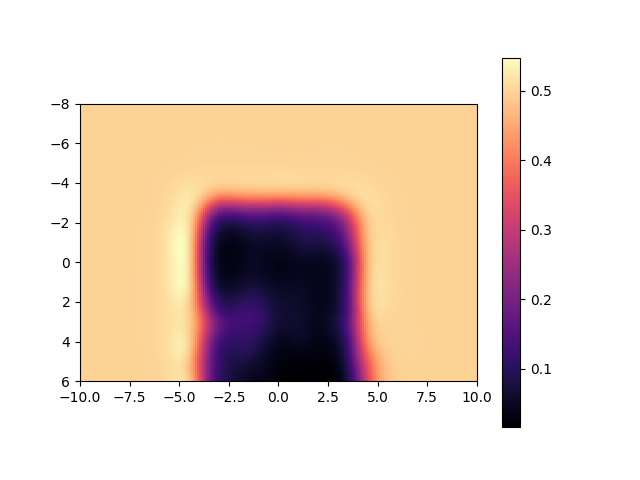
\includegraphics[width=75mm,trim={0 14mm 0
    10mm},clip]{Chap4/fig/ten_x_-1}}}%
    \hfill \subfloat[Plane
    $z=-2$]{{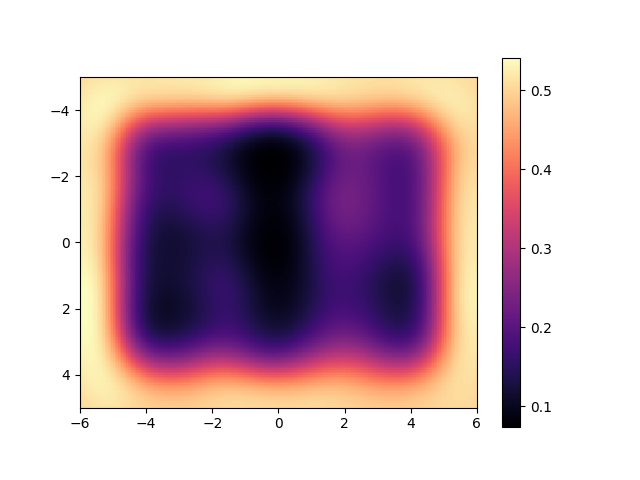
\includegraphics[width=75mm,trim={0 14mm 0
    10mm},clip]{Chap4/fig/ten_z_-2}}}%
    \\%
    \subfloat[Plane
    $x=0$]{{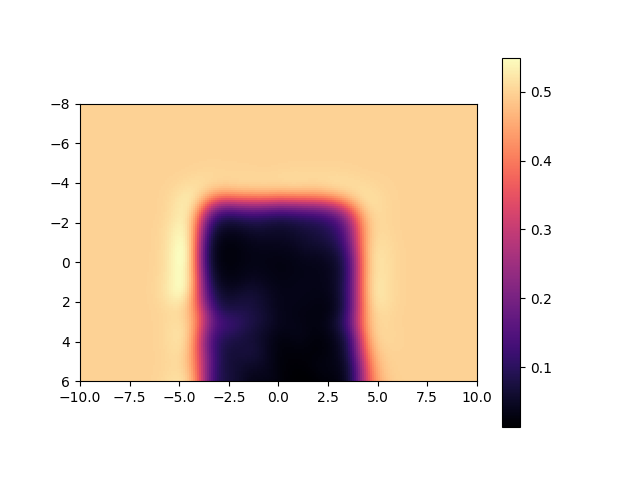
\includegraphics[width=75mm,trim={0 14mm 0
    10mm},clip]{Chap4/fig/ten_x_0}}}%
    \hfill \subfloat[Plane
    $z=-1$]{{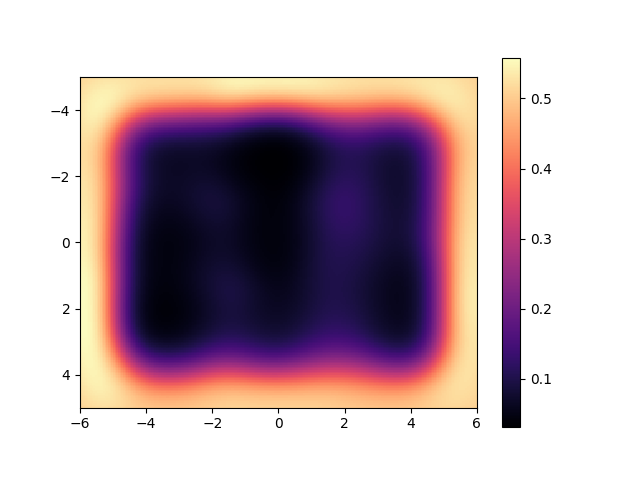
\includegraphics[width=75mm,trim={0 14mm 0
    10mm},clip]{Chap4/fig/ten_z_-1}}}%
    \\%
    \subfloat[Plane
    $x=1$]{{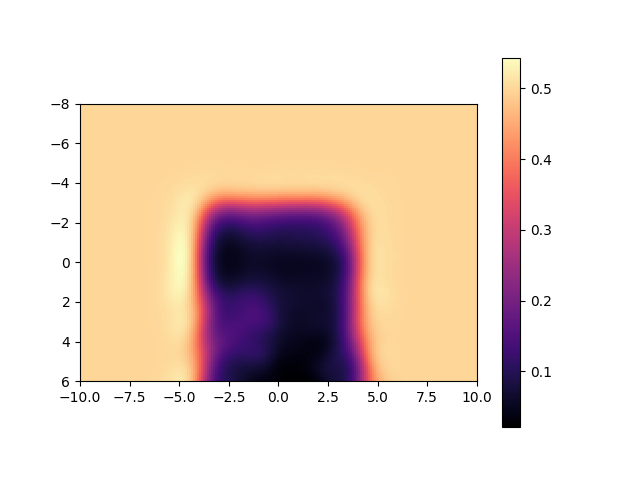
\includegraphics[width=75mm,trim={0 14mm 0
    10mm},clip]{Chap4/fig/ten_x_1}}}%
    \hfill \subfloat[Plane
    $z=0$]{{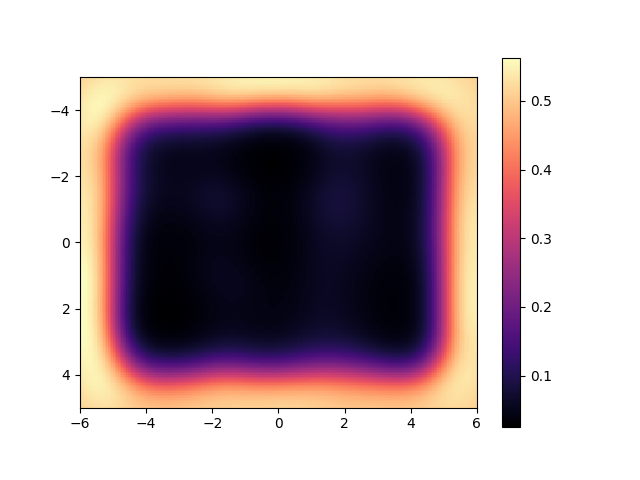
\includegraphics[width=75mm,trim={0 14mm 0
    10mm},clip]{Chap4/fig/ten_z_0}}}%
    \caption{Mapping with $10\%$ of available beams.}%
    \label{fig:ten_map}%
\end{figure}

\begin{figure}[ht]
    \centering
    \subfloat[Plane
    $x=-1$]{{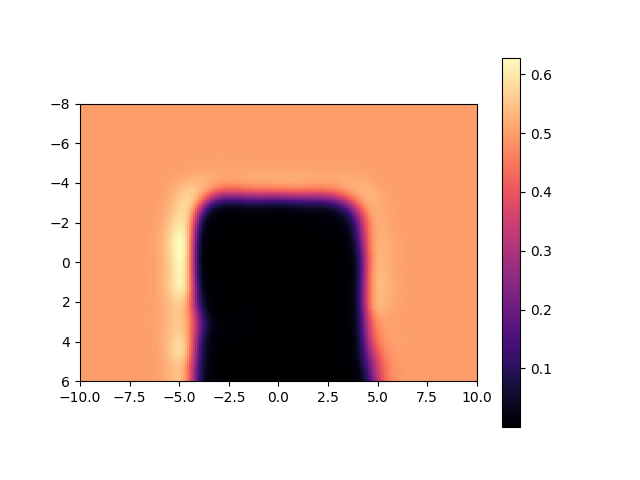
\includegraphics[width=75mm,trim={0 14mm 0
    10mm},clip]{Chap4/fig/thir_x_-1}}}%
    \hfill \subfloat[Plane
    $z=-2$]{{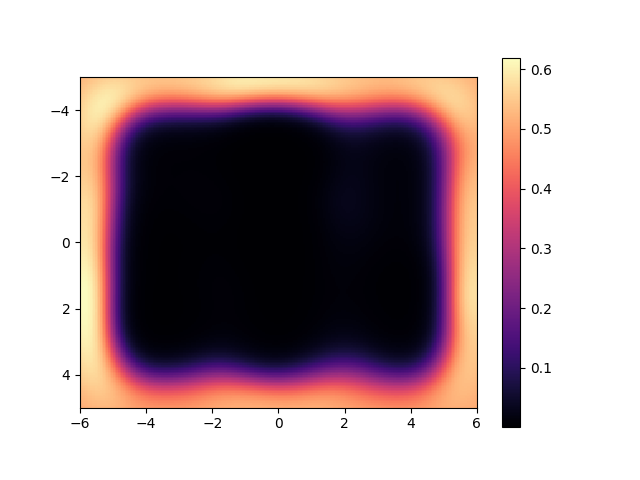
\includegraphics[width=75mm,trim={0 14mm 0
    10mm},clip]{Chap4/fig/thir_z_-2}}}%
    \\%
    \subfloat[Plane
    $x=0$]{{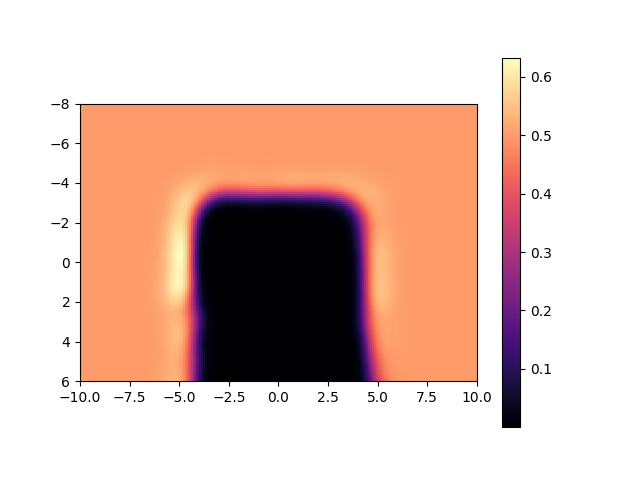
\includegraphics[width=75mm,trim={0 14mm 0
    10mm},clip]{Chap4/fig/thir_x_0}}}%
    \hfill \subfloat[Plane
    $z=-1$]{{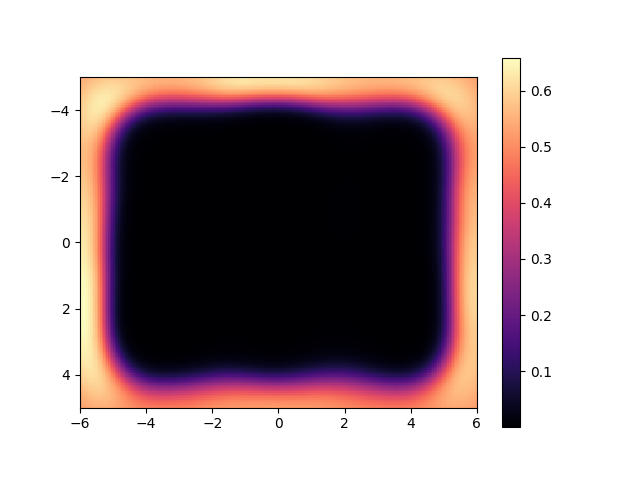
\includegraphics[width=75mm,trim={0 14mm 0
    10mm},clip]{Chap4/fig/thir_z_-1}}}%
    \\%
    \subfloat[Plane
    $x=1$]{{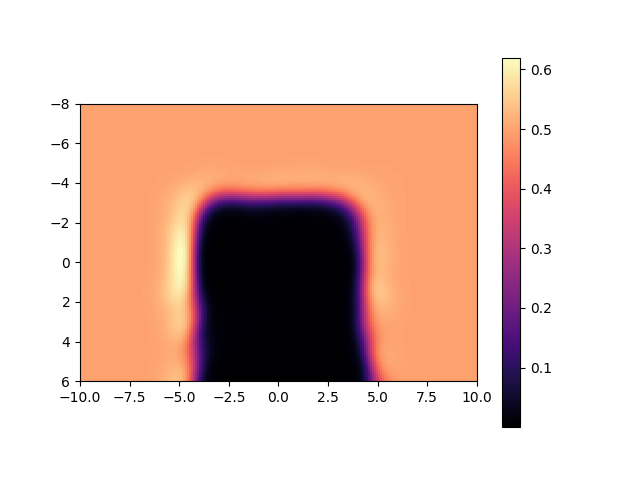
\includegraphics[width=75mm,trim={0 14mm 0
    10mm},clip]{Chap4/fig/thir_x_1}}}%
    \hfill \subfloat[Plane
    $z=0$]{{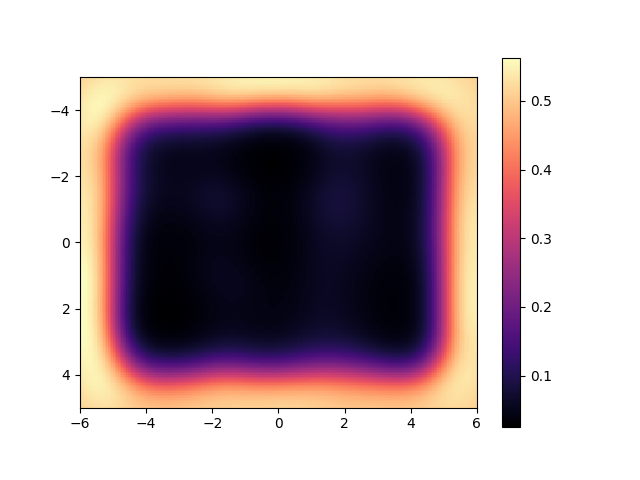
\includegraphics[width=75mm,trim={0 14mm 0
    10mm},clip]{Chap4/fig/ten_z_0}}}%
    \caption{Mapping with $30\%$ of available beams.}%
    \label{fig:thir_map}%
\end{figure}

\begin{figure}[ht]
    \centering
    \subfloat[Plane
    $x=-1$]{{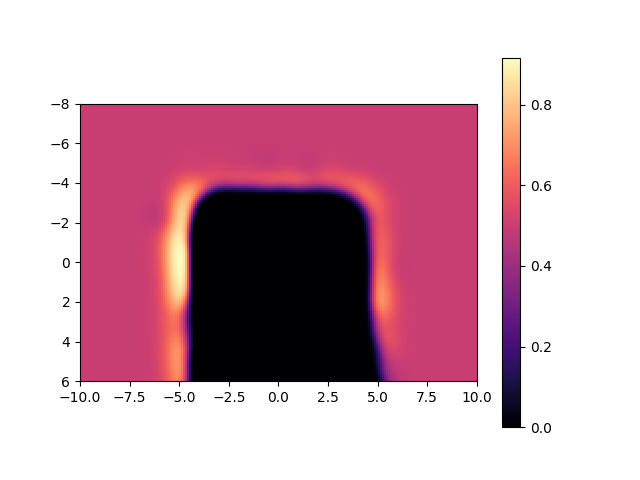
\includegraphics[width=75mm,trim={0 14mm 0
    10mm},clip]{Chap4/fig/full_x_-1}}}%
    \hfill \subfloat[Plane
    $z=-2$]{{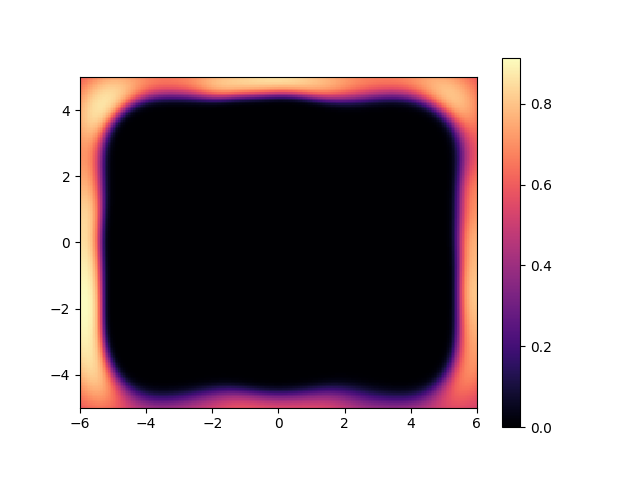
\includegraphics[width=75mm,trim={0 14mm 0
    10mm},clip]{Chap4/fig/full_z_-2}}}%
    \\%
    \subfloat[Plane
    $x=0$]{{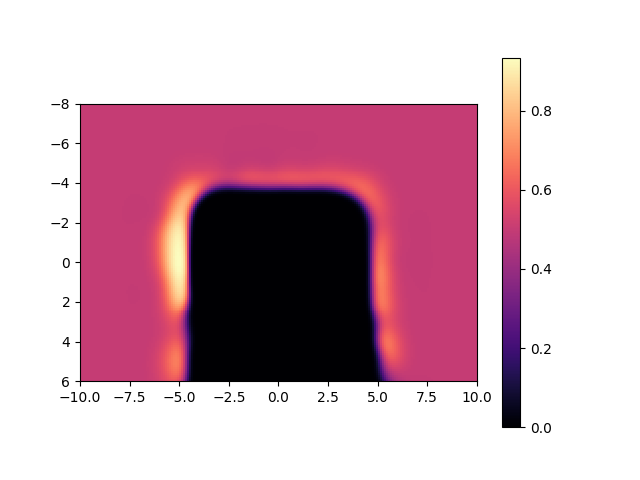
\includegraphics[width=75mm,trim={0 14mm 0
    10mm},clip]{Chap4/fig/full_x_0}}}%
    \hfill \subfloat[Plane
    $z=-1$]{{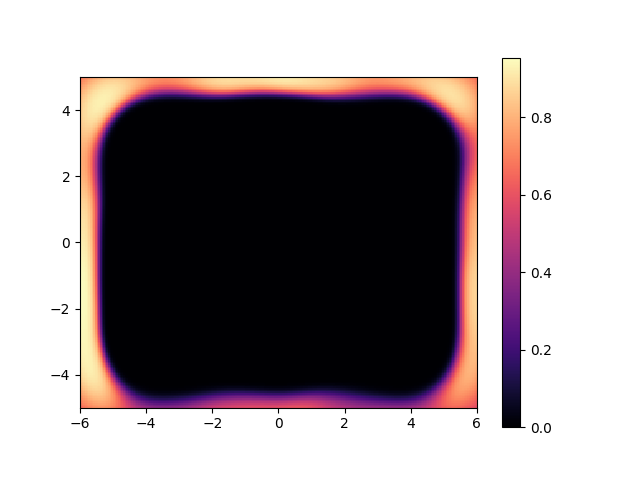
\includegraphics[width=75mm,trim={0 14mm 0
    10mm},clip]{Chap4/fig/full_z_-1}}}%
    \\%
    \subfloat[Plane
    $x=1$]{{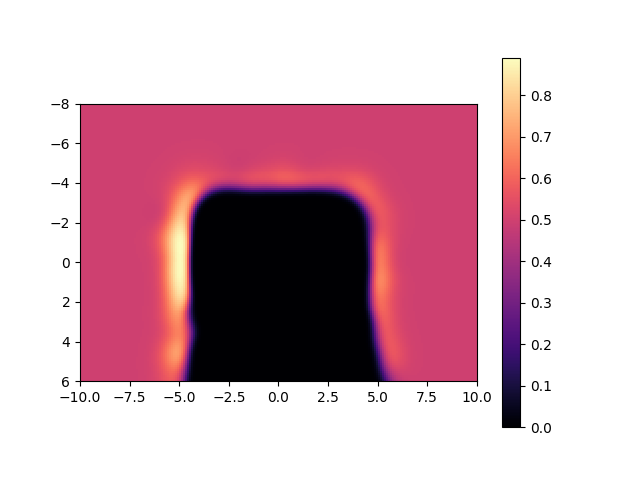
\includegraphics[width=75mm,trim={0 14mm 0
    10mm},clip]{Chap4/fig/full_x_1}}}%
    \hfill \subfloat[Plane
    $z=0$]{{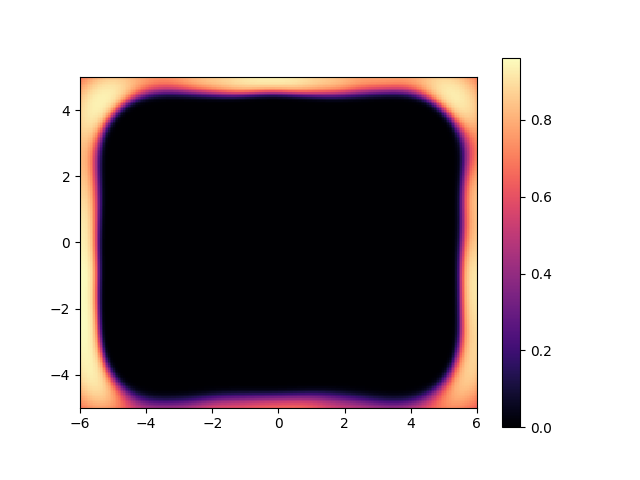
\includegraphics[width=75mm,trim={0 14mm 0
    10mm},clip]{Chap4/fig/full_z_0}}}%
    \caption{Mapping with $100\%$ of available beams.}%
    \label{fig:full_map}%
\end{figure}


\chapter{Mathematical Preliminaries}

Some of the more advanced mathematical tools\footnote{As judged by the autor
from the perspective of a graduated student.} used on the development of this
thesis are presented here.
Other knowledges, as basic linear algebra and analysis, are take as granted.


\section{Hilbert Space}
\label{s:hilbert}
A Hilbert Space is a complete inner product space \cite{HS-YN:11}. It is a
complete metric space with respect to the metric induced by its inner product
(which in turn can be thought indirectly by its induced norm). A nice picture
is as a generalization of the Euclidean space. Which means intuition works well,
in contrast with the broader concept of Banach Spaces, a complete normed space,
where the infinite dimensional case can be quite different from what one would
expect\footnote{Banach Space are complete metric spaces where the metric does
not come necesserally from a inner product. (See \citet{HS-HJNB:00})}.

An inner product space\cite{HS-HJNB:00} is a (possibly infinite dimensional)
vector space $V$ over $\mathbb{C}$ (or $\mathbb{R}$ by restriction ), together
with a map (called the \textbf{inner product}):

\[  \langle\cdot,\cdot\rangle_{\scriptscriptstyle V}: V \times V \to \mathbb{C}
\]

Satisfing the following properties, for all $x,y,z \in V$ and all $\mu, \lambda
\in \mathbb{C}$:

\begin{enumerate}[I]
  \item \(  \langle x,\lambda y + \mu z  \rangle_{\scriptscriptstyle V} = \lambda\langle	
  x,y\rangle_ {\scriptscriptstyle V} + \mu \langle x,z \rangle_{\scriptscriptstyle V} \) (linear in the second argument)
  \item \( \langle x,y \rangle_{\scriptscriptstyle V} = \overline{\langle y,x \rangle_{\scriptscriptstyle V} } \)
  (Hermitian symmetric)
  \item  \( \langle x,x \rangle_{\scriptscriptstyle V} \geq 0 \) and \( \langle x,x \rangle_{\scriptscriptstyle V} = 0
  \Leftrightarrow x = 0 \) (positive definite)
\end{enumerate}

A classical example of a inner product is the euclidean dot product.

Another important example is the inner product defined on the space C$[a,b]$ of
complex (or real) valued continuous functions on the interval $[a,b]$, defined,
for every $f$ and $g$ in C$[a,b]$ as:

\begin{equation}\label{eq::func_inner}
  \langle f,g\rangle_{\scriptscriptstyle \text{C}[a,b]} = \int_a^b
  f(x)\overline{g(x)} \mathrm{d}x
\end{equation}

On any Hibert Space $\hs$ the norm induced by the inner product is:

\begin{equation}
  \hnorm{x} = \sqrt{ \hip{x}{x} }
\end{equation}

where $x \in \hs$. And the subsequent metric is defined as:

\begin{equation}\label{eq::norm_metric}
  d_{_\hs}(x,y) = \hnorm{ x - y }
\end{equation}

for any $x,y \in \hs$.

A vector space endowed with a inner product is a \textit{inner product space}
(aka. pre-Hilbert space). For it to be a Hibert Space it also has to be complete
with respect to the above metric. Completeness means that any Cauchy sequence
converges in this space (which provides a suitable framework to apply the tools
of calculus). A Cauchy sequence is a sequence where every term becomes
arbitrarily close to each other as the sequence progress (not only to term
right next to it). It can be formalized as the sequence
$x_1$,$x_2$,$x_3$,$\ldots$ on a metric space (with a metric $d( \cdot ,\cdot)$)
where:


\[ \forall \epsilon \in \mathbb{R}^+, ~\exists N \in \mathbb{Z}^+, ~\forall
n,m>N \Longrightarrow ~d(x_n,x_m)<\epsilon
\]

On a pre-Hilbert space, the metric is given by equation \ref{eq::norm_metric}.
If a metric space $M$ is complete, then every Cauchy sequence
($x_1$,$x_2$,$x_3$,$\ldots$) converges in that space:

\[ \exists x \in M, \forall \epsilon \in \mathbb{R}^+, ~\exists N \in \mathbb{Z}^+, ~\forall
n>N \Longrightarrow ~d(x_n,x)<\epsilon
\]
So,
\[ x = \lim_{n\to\infty} x_n \]

A complete metric space can be obtained from a pre-Hilbert space, by completion,
in the same way that $\mathbb{Q}$ is ``completed'' to make $\mathbb{R}$.
Although completeness is a technicality, it is easy to find examples of
pre-Hibert spaces that lacks this property. The space of continuous functions
C$[a,b]$ with the inner product defined on \ref{eq::func_inner} gives an example
of pre-Hibert space that is not complete. For it to be a Hilbert space, the
space have to be extend to include some discontinuous functions, as in the larger
set of Lebesgue mensurable\footnote{The Lebesgue mensurability of a, bounded
with compact support, function is a highly technical exigence and the existence
of a bounded non-Lebesgue mensurable set (which allow the construction of such a
function) is dependent on the axiomatic choice of the underlying set theory - it
can only be proven with the adition of the \textit{choice axiom} to the
ZF (Zermelo-Fraenkel) set of axioms (ZFC). } functions that are square
integrable (with the Lebesgue integral).

Some examples of Hilbert space are:

\begin{itemize}
  \item Any finite dimensional vector space over the field $\mathbb{R}$ or
  $\mathbb{C}$ with the standard dot product.
  \item The space $\ell^2$ of square-summable sequences of complex numbers, i.e.
  $(c_1,c_2,c_3,\ldots)$ with $c_i \in \mathbb{C}$ and $\sum_{i=1}^\infty |c_i|^2 <
  \infty$, is a Hilbert space with the inner product defined as: Given two
  sequences $x=(x_1,x_2,x_3,\ldots)$ and $y=(y_1,y_2,y_3,\ldots)$, define $\langle x,y
  \rangle_{\scriptscriptstyle \ell^2} = \sum_{i=1}^\infty x_i \bar{y_i}$.
  \item Fourier series can be seen as the representation of a square-integrable
  function on the interval $[0,1]$ (member of $L^2[0,1]$) on the orthogonal
  basis $\{\mathrm{e}^{2\pi i n \theta} : n \in \mathbb{Z}\}$ with the
  inner product given by \ref{eq::func_inner}.
\end{itemize}


\section{RKHS - Reproducing Kernel Hilbert Space}
\section{Probabilistic Regression}
\backmatter
\bibliographystyle{formating/coppe-unsrt}
\bibliography{biblio}

\end{document}
